\documentclass[journal]{vgtc} 
\usepackage{hs-vis_ws1819}
\usepackage{url}


%% Please note that the use of figures other than the optional teaser
%% is not permitted on the first page of the journal version.  Figures
%% should begin on the second page and be in CMYK or Grey scale
%% format, otherwise, colour shifting may occur during the printing
%% process.  Papers submitted with figures other than the optional
%% teaser on the first page will be refused.

%% These three lines bring in essential packages: ``mathptmx'' for
%% Type 1 typefaces, ``graphicx'' for inclusion of EPS figures. and
%% ``times'' for proper handling of the times font family.

\usepackage{mathptmx} 
\usepackage{graphicx}
\usepackage{times}
\usepackage[space]{grffile}
\usepackage{hyperref}


%% allow for this line if you want the electronic option to work
%% properly
\vgtcinsertpkg


%% author name
\author{Dominik Sellenthin \and Michael Stegmaier \and Gariharan Kanthasamy}

%% paper title
\title{OpenGL-basiertes Software Occlusion Culling zur Beschleunigung des 3D-Renderings gro{\ss}er Datenmengen und komplexer Szenen}

%% short title for header
\shorttitle{Software Occlusion Culling}


%% Abstract section.
\abstract{%

%%% ÜBERARBEITUNG BENÖTIGT %%%
In Bereichen des 3D-Rendering, sei es in der wissenschaftlichen Visualisierung oder in Computerspielen, ist die Rechenleistung der Grafikkarte schnell an ihrer Grenze, w"ahrend die CPU kaum in Anspruch genommen wird. Es werden daher Techniken ben"otigt, die den Aufwand beim Rendern so gering wie m"oglich halten und gleichzeitig der st"andig zunehmenden Dynamik gerecht werden. Eine dieser Techniken ist das Software Occlusion Culling (SOC). Ziel des Occlusion Cullings ist es, komplett parallel zum GPU-Rendering des aktuellen Frames, festzustellen, welche Objekte in der kommenden Szene zu sehen sind und welche Objekte nicht gerendert werden m"ussen. Damit die GPU entlastet wird, ist es W"unschenswert, die Berechnungen des Occlusion Cullings auf die CPU auszulagern. Um das zu erreichen und um die vollst"andige Rechenleistung moderner Multi-Core CPUs zu gew"ahrleisten, wird in dieser Arbeit ein bereits vorhandener Software-Rasterierer, Mesa 3D, verwendet, der zus"atzlich die OpenGL API zur Verf"ugung stellt. In dieser Arbeit wird daher in einem von Intel entwickelten SOC-Framework eine auf Mesa-3D basierende Occlusion Culling Technik implementiert und folglich auf ihre Tauglichkeit mit bereits im Framework existierenden Techniken verglichen.
} % end of abstract


%% Uncomment below to include a (optional) teaser figure.
\teaser{ \centering
  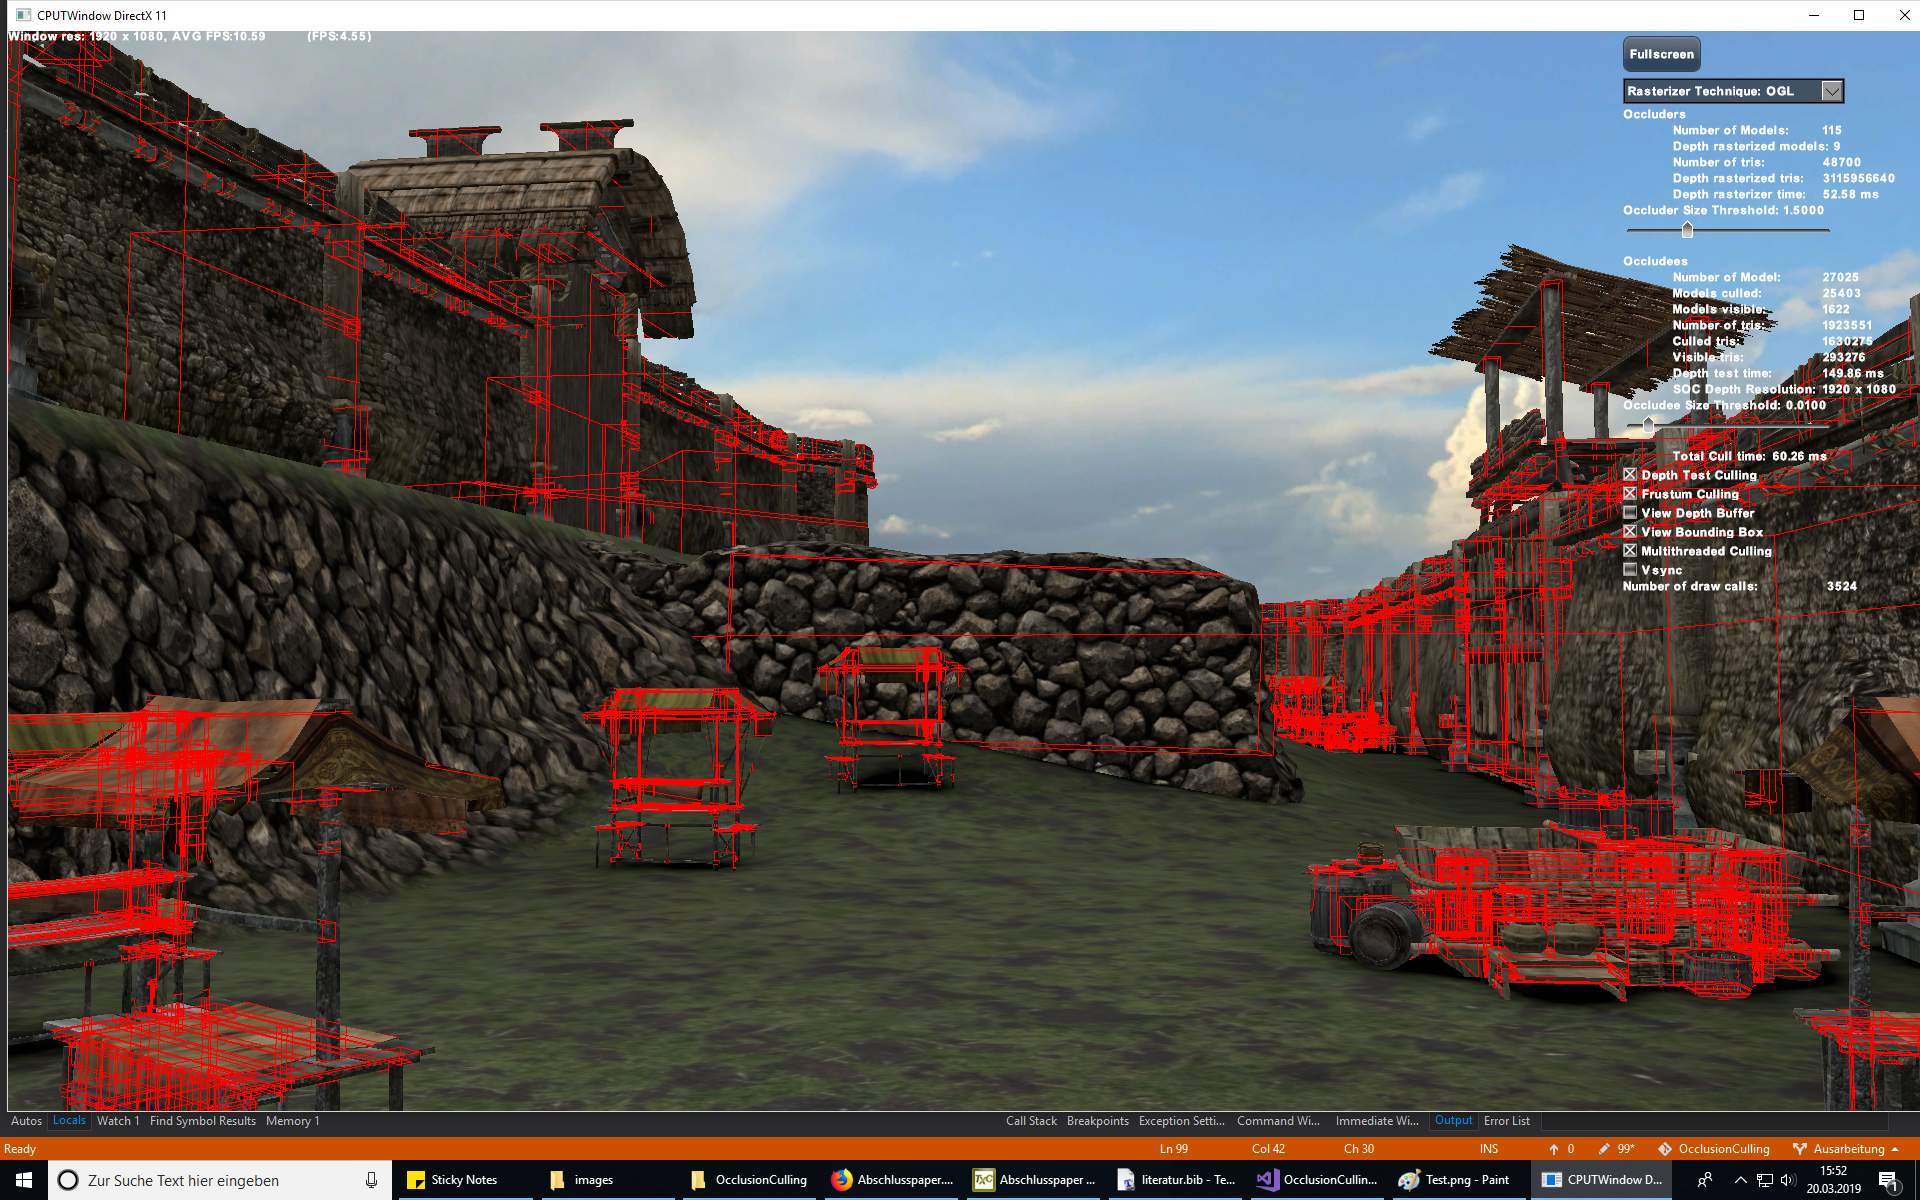
\includegraphics[width=\columnwidth]{images/Base1AABB.png}%
	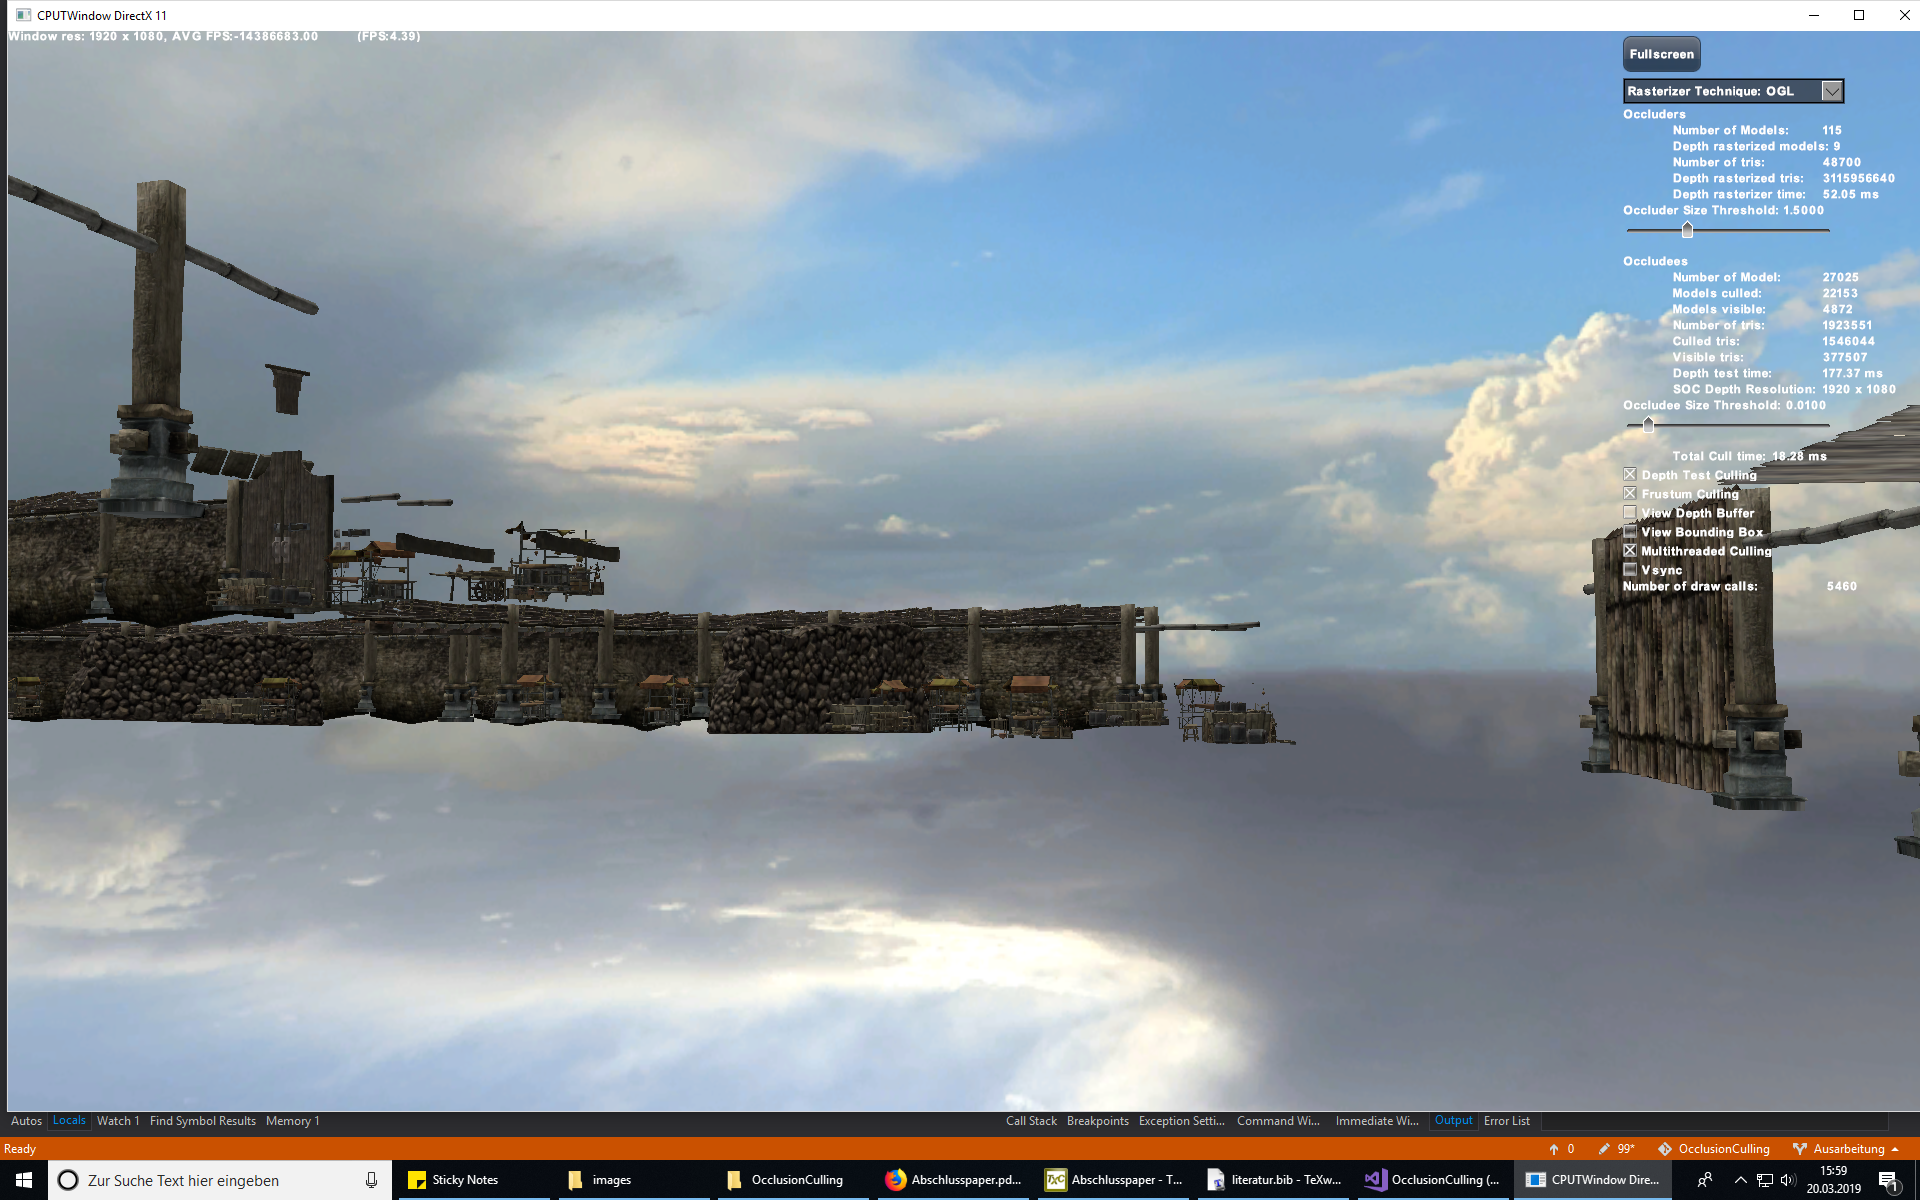
\includegraphics[width=\columnwidth]{images/Base1Invert.png}%
	\caption{Links: Testergebnisbild nach einem erfolgreichen Durchlauf der OGL-Methode aus der verwendeten Intel-Testszene. Rote Linien um Objekte stellen die Axis Aligned Bounding Box des jeweiligen Objekts dar. Rechts: Bild aller Objekte, die beim Occlusion Culling als verdeckt klassifiziert wurden und im linken Bild nicht gerendert wurden.}%
	\label{fig:teaser}
}


%%%%%%%%%%%%%%%%%%%%%%%%%%%%%%%%%%%%%%%%%%%%%%%%%%%%%%%%%%%%%%%%
%%%%%%%%%%%%%%%%%%%%%% START OF THE PAPER %%%%%%%%%%%%%%%%%%%%%%
%%%%%%%%%%%%%%%%%%%%%%%%%%%%%%%%%%%%%%%%%%%%%%%%%%%%%%%%%%%%%%%%

\begin{document}

%% The ``\maketitle'' command must be the first command after the
%% ``\begin{document}'' command. It prepares and prints the title
%%   block.

%%   the only exception to this rule is the \firstsection command
\firstsection{Einleitung}

\maketitle

Heutige Anwendungen haben immer h"ohere Anspr"uche an die Leistung der Engines(?) und der Wunsch nach besserer Performanz und h"oheren Bildraten (frames per second, FPS) ist gro{\ss}. Hinzukommt, dass in modernen Anwendungen die zu rendernden Szenen immer weniger statisch und immer mehr dynamisch werden, wie es beispielsweise in Computerspielen der Fall ist. Um dieser Dynamik gerecht zu werden, wird sich von Verfahren mit potenziellen Sichtbarkeitsmengen entfernt \cite{MSOC} und es wird sich einer Methode namens \textit{Occlusion Culling} (\textit{to occlude = verdecken, to cull = aussondern, herausfiltern}) bedient. Ziel des Occlusion Cullings ist es, noch vor dem Rendering der n"achsten Szene, herauszufinden, welche Objekte in der kommenden Szene sichtbar sind und welche nicht. Im Wesentlichen gilt es dabei zuerst mit einer ausgew"ahlten Teilmenge der Objekte einen geeigneten Tiefenpuffer (Z-Buffer) zu generieren und darauffolgend mit Hilfe von Occlusion Queries alle Objekte zu bestimmen, die noch sichtbar sind (auch Z-Buffering oder Tiefentest genannt). Das Ergebnis der Occlusion Queries kann anschlie{\ss}end ohne nennenswerte Latenz verwendet werden, um der GPU mitzuteilen, welche Objekte gerendert werden sollen, so dass unn"otiger Rechenaufwand der GPU vermieden wird.

Bei Anwendungen, die ohnehin schon enormen Rechenaufwand ben"otigen und die maximale Rechenkapazit"at der Grafikkarte schnell ausreizen, ist es schwierig den zus"atzlichen Mehraufwand ebenfalls der Grafikkarte aufzuerlegen. Es bietet sich daher an, den Mehraufwand dem wenig genutzten Prozessor zu "ubergeben, der dann komplett parallel zur Grafikkarte das Occlusion Culling in einem Vorverarbeitungsschritt durchf"uhren soll, siehe Abb.\ \ref{fig:ablauf}.

\begin{figure}%
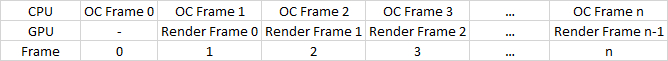
\includegraphics[width=\columnwidth]{images/Ablauf.PNG}%
\caption{Prozessor berechnet parallel zum Rendering der Grafikkarte, welche Objekte in der n"achsten Szene zu sehen sind.}%
\label{fig:ablauf}%
\end{figure}

Moderne Prozessoren besitzen mittlerweile einige separat nutzbare Kerne, die parallel verwendet werden k"onnen, um das Occlusion Culling so effektiv und effizient wie m"oglich zu implementieren. Damit die gesamte Rechenleistung der Prozessoren auch genutzt wird, wird in dieser Arbeit auf den Software-Rasterisierer Mesa 3D zur"uckgegriffen, der au{\ss}erdem mit der bew"ahrten OpenGL API arbeitet. 

Implementiert wurde die OGL-Methode in einem Software Occlusion Culling (SOC) Framework, das von Intel frei zur Verf"ugung gestellt wird \cite{SOCF}. Das Framework eignet sich sehr gut f"ur die Implementierung einer neuen SOC-Methode, da es sowohl essentielle Ablaufstrukturen als auch eine ausreichend gro{\ss}e und komplexe Testszene zur Verf"ugung stellt, mit der eine Evaluation der OGL-Methode erm"oglicht wird, siehe Abb.\ \ref{fig:teaser} links.


\section{Related Work}
Diese Arbeit orientiert sich stark an Intels SOC-Framework, in das die in dieser Arbeit entwickelte OGL-Methode eingebettet wurde. Da das Framework bereits alle notwendigen Strukturen f"ur schon bestehende Methoden besitzt (siehe Abb.\ \ref{fig:ablaufframework}), gestaltet sich die Erweiterung um eine weitere Methode gr"o{\ss}tenteils unkompliziert. 
\begin{figure}%
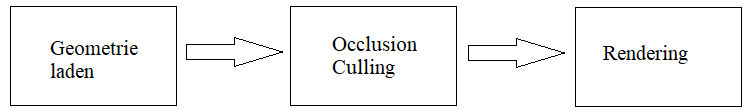
\includegraphics[width=\columnwidth]{images/AblaufFramework.png}%
\caption{Verwende gr"o{\ss}tenteils vorhandene Strukturen, um die verwendete Geometrie zu laden. Anschlie{\ss}end erfolgt das Culling durch die neue OGL-Culling-Methode. Zum Schluss wird die nicht gecullte Geometrie an das Framework zur"uckgegeben, damit das Ergebnis gerendert wird.}%
\label{fig:ablaufframework}%
\end{figure}
Hinzukommen lediglich Ver"anderungen der Routinen zum Laden der Testszene und die Implementierung des Cullings selber. Vorhanden sind unter anderem Methoden, die mit \textit{Streaming SIMD Extension} (SSE) und \textit{Intel Advanced Vector Extension} (AVX) arbeiten. Au{\ss}erdem ist noch eine optimierte Variante der AVX-Technik vorhanden, \textit{Masked Software Occlusion Culling} (MSOC) \cite{MSOC}, die mit einer abgewandelten Form des hierarchischen Z-Buffers (HiZ) \cite{HiZ} arbeitet, der durch einen Software-Rasterisierer berechnet wird.

Hasselgren et al. \cite{MSOC} stellen in ihrer Arbeit einen Algorithmus vor, der durch seinen effizienten HiZ die Performanz signifikant verbessert. Anstatt wie in fr"uheren Arbeiten Pixel als kleinste Einheit zu betrachten, werden nun \textit{Kacheln} verwendet. Kacheln sind dabei lediglich eine Zusammenfassung mehrerer aneinanderliegender Pixel. Da AVX2 erm"oglicht, 8 SIMD Instruktionen mit 32-Bit Pr"azision auszuf"uhren, wurde f"ur die Kacheln eine Gr"o\ss{}e von 32x8 Pixeln gew"ahlt. Indem Bitmasken von rechts und links in die Kacheln geschoben werden, wird am Ende eine Abdeckungsmaske erhalten, die angibt, welche Pixel in einer Kachel verdeckt werden \cite{MSOC}.
W"ahrend ihr Algorithmus keine 100\% Pr"azision garantiert - \textit{false positives} sind m"oglich - bewegt sich der Fehler in gleicher Gr"o\ss{}enordnung wie bei bisherigen Algorithmen. Ein wichtiger Faktor f"ur die Performanz ihres Algorithmus ist die Reihenfolge, in der die Objekte gerendert werden. Die Objekte sollten bestm"oglichst von vorne nach hinten gerendert werden. Dadurch werden die wichtigsten Occluder als erstes rasterisiert (dargestellt) und f"ur den Fall, dass die Zeit f"ur Occlusion Culling begrenzt ist, wird trotzdem ein nahezu optimales Ergebnis erzielt \cite{MSOC}.

Bei einem Vergleich zwischen einem HiZ-Algorithmus und dem MSOC - bei voller Aufl"osung (1920*1080 Pixel) und Single-Core Performanz - geht hervor, dass der MSOC-Algorithmus 2\% weniger Dreiecke als der HiZ wegwirft, aber dennoch eine bessere Performanz erzielt. Mit beiden Occlusion Culling Algorithmen kann eine 1,5-7x schnellere Total Frame Time gegen"uber Rendering mit nur Frustumculling erreicht werden. In einem zweiten Test in einer wesentlich komplexeren Szene mit 143k Occluder-Meshes ist die Occlusion Culling Time des MSOC-Algorithmus zeitweise bis zu 10x schneller als die des HiZ-Algorithmus. Die Skalierbarkeit des MSOC is der des HiZ deutlich "uberlegen. Mit steigender Gr"o"se der Dreiecke steigt auch der Performanzunterschied zwischen dem MSOC und dem HiZ. Im Allgemeinen soll der MSOC-Algorithmus 3x schneller sein und gleichzeitig 98\% aller Dreiecke wegwerfen als die bisherigen Algorithmen bei einem nur geringen Memory Overhead.



\section{Software Occlusion Culling}
Die Menge der Objekte, die es zu Rendern gilt, wird in zwei Mengen aufgeteilt. Zum einen gibt es die \textit{Occluder}. Occluder sind eine Menge von Objekten, die gro{\ss} genug sind, dass es wahrscheinlich ist, dass sie andere Objekte verdecken. Zum anderen gibt es \textit{Occludees}. Occludees sind all diejenigen Objekte die potenziell von Occludern verdeckt werden (das hei{\ss}t, sie beinhalten ebenfalls alle Occluder).
\begin{figure}%
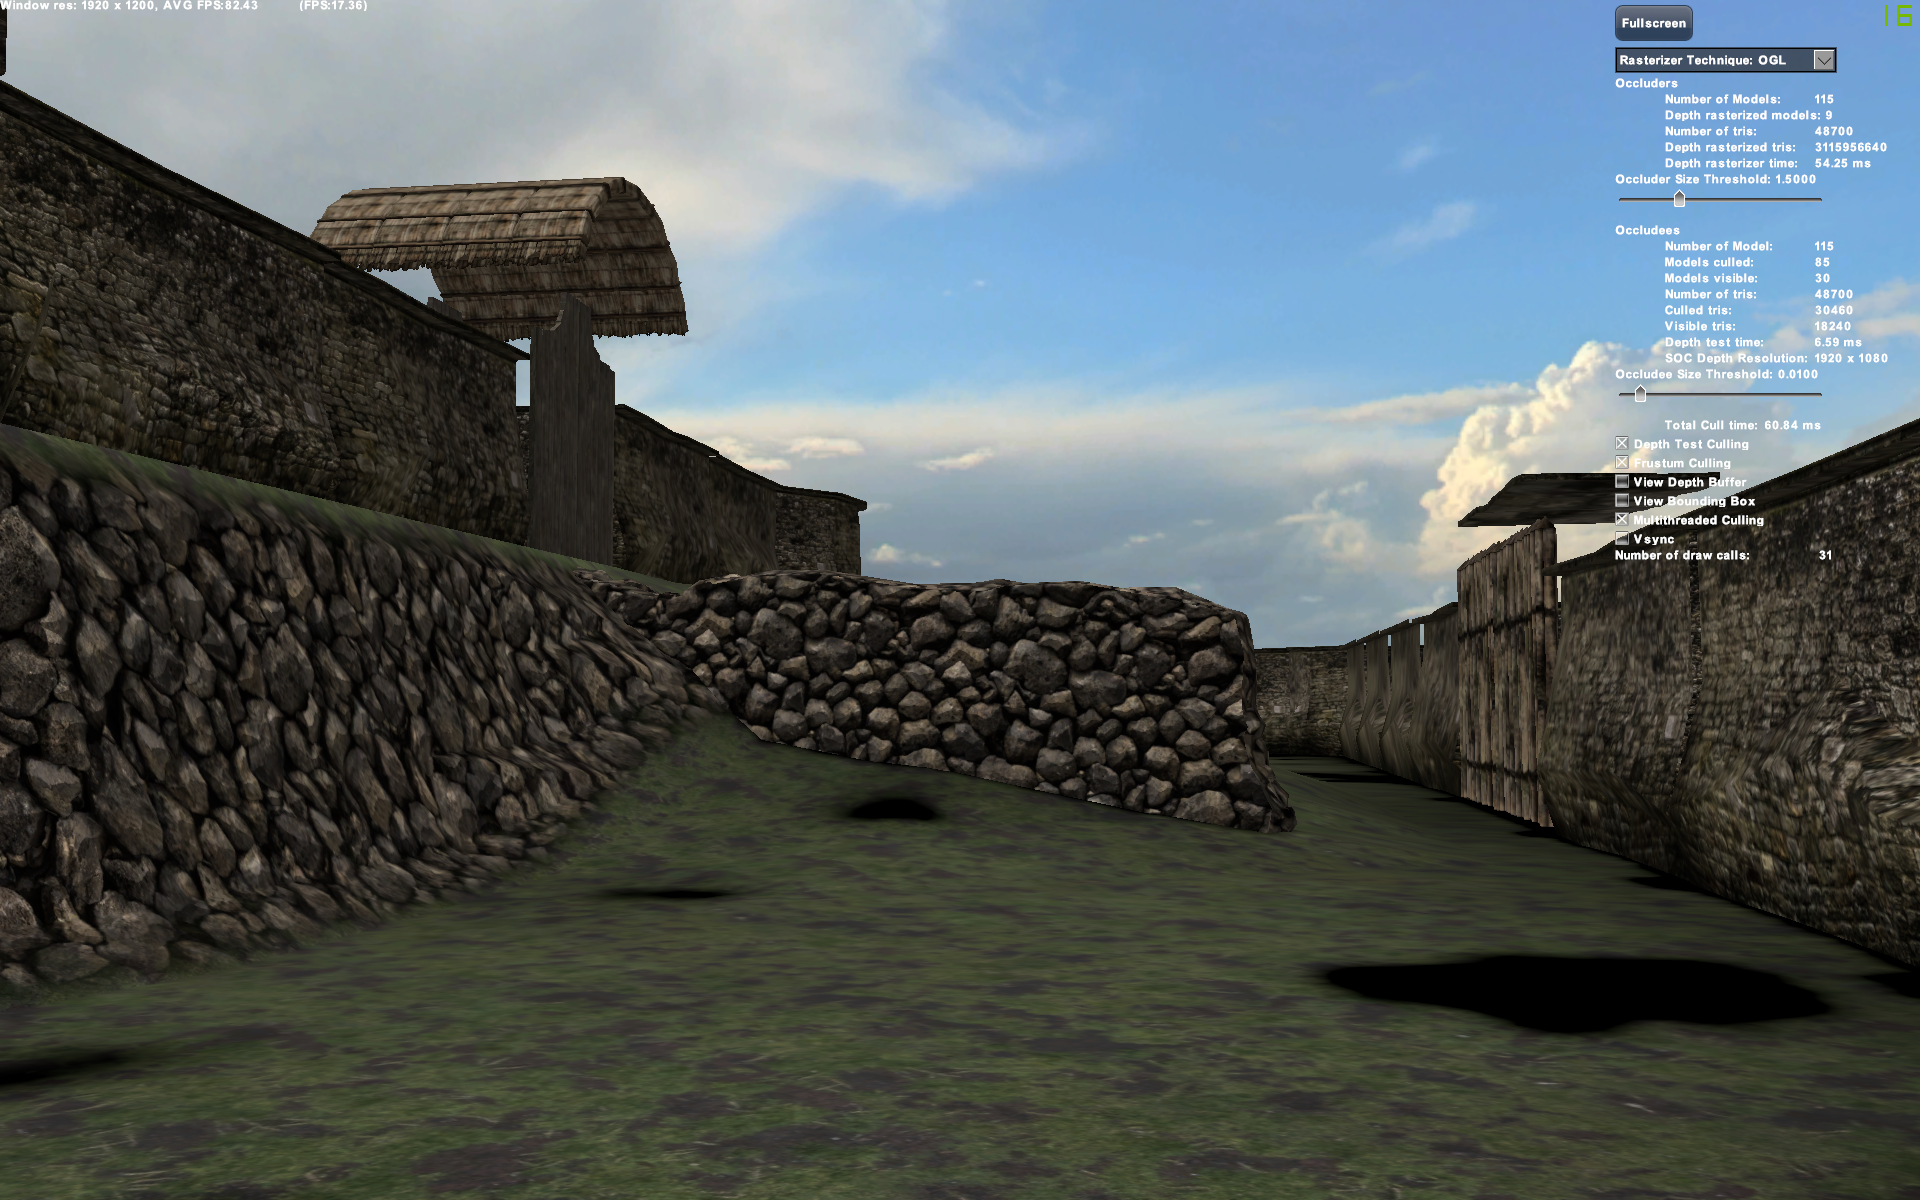
\includegraphics[width=0.5\columnwidth]{images/Occluder.png}%
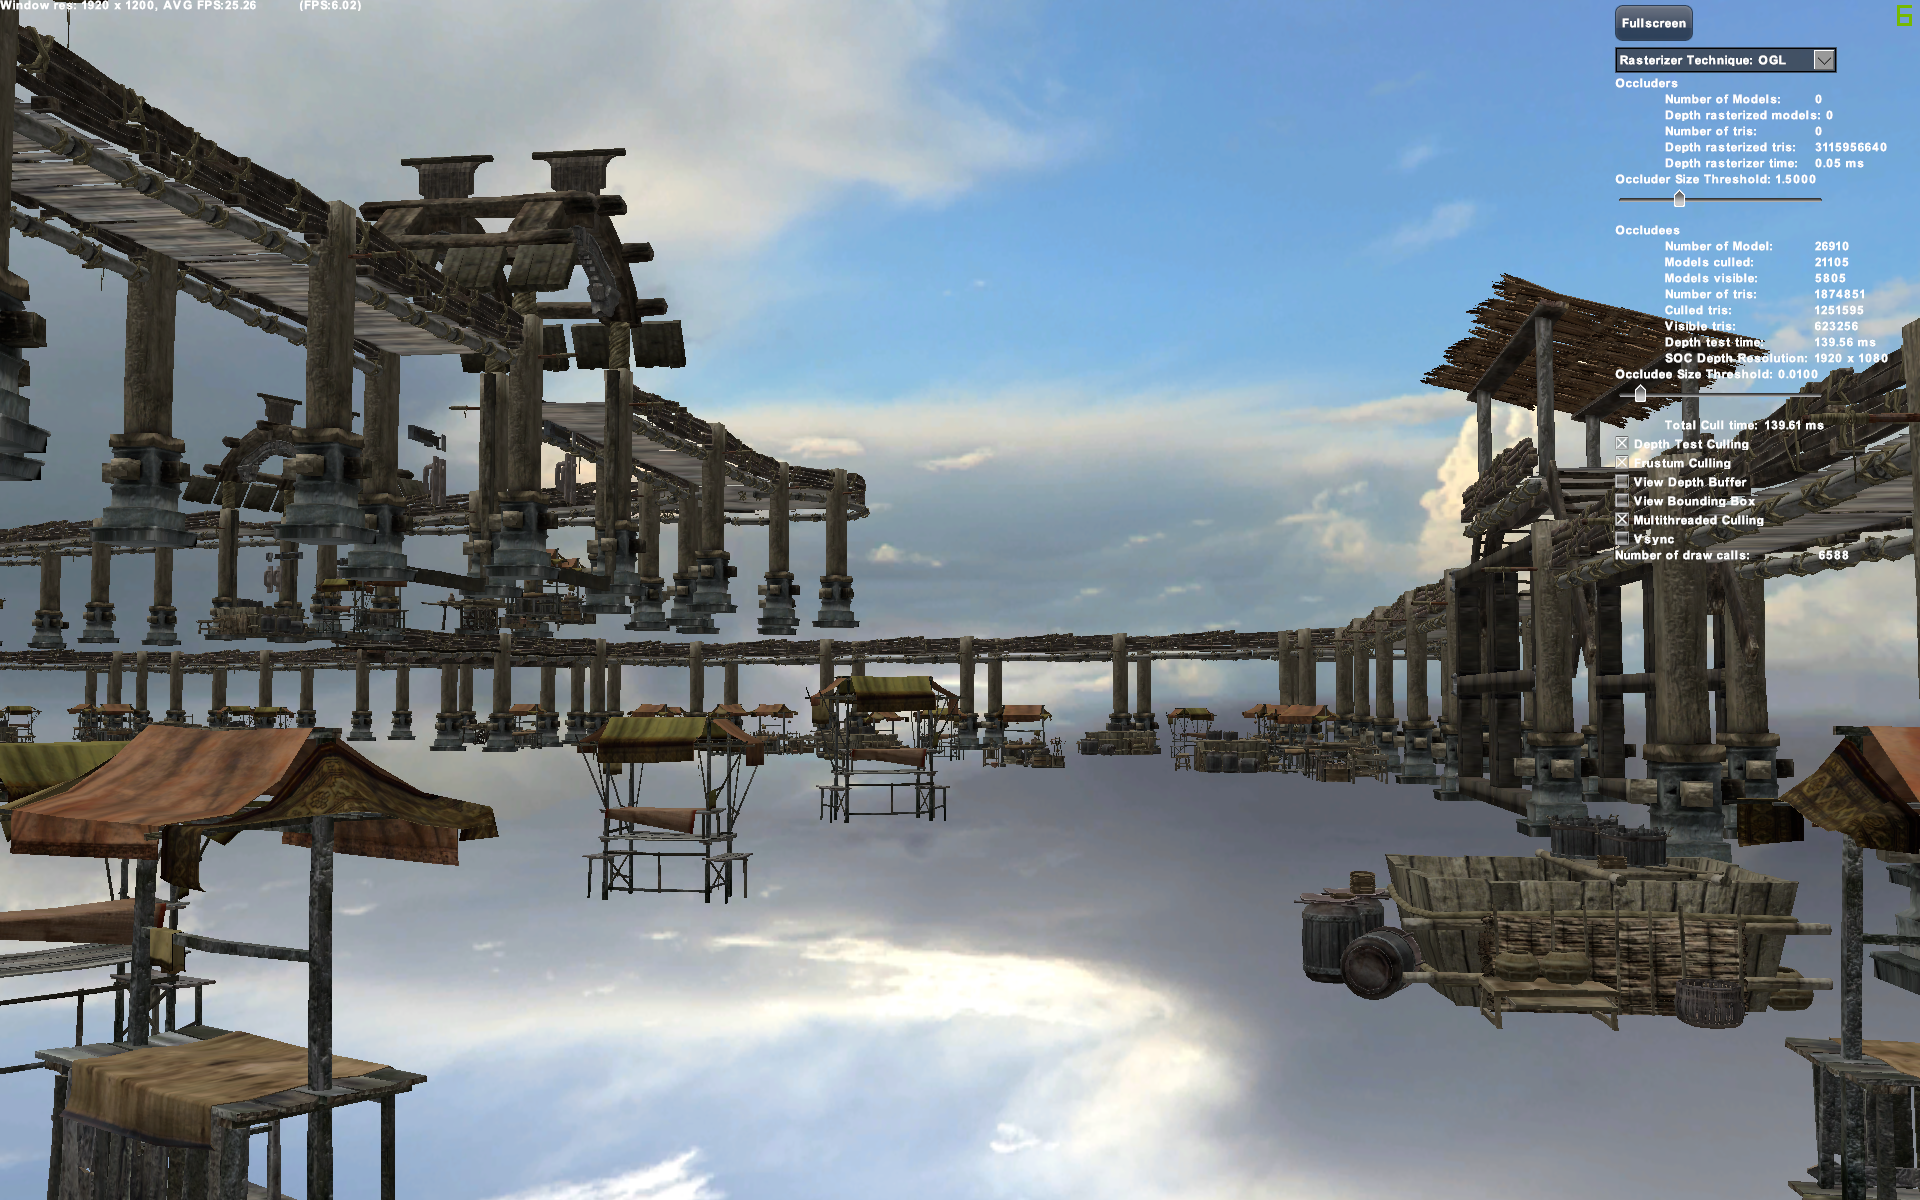
\includegraphics[width=0.5\columnwidth]{images/Occludees.png}%
\caption{Links: Menge der Occluder ohne Occludees, die in dieser Kameraeinstellung zu sehen sind, vgl. Abb.\ \ref{fig:teaser} linkes Bild. Rechts: Testszene ohne Occluder, es sind ausschlie{\ss}lich Occludees zu sehen, vgl. ebenfalls Abb.\ \ref{fig:teaser}.}%
\label{fig:objects}%
\end{figure}
 Sowohl Occluder als auch Occludees liegen dabei in zwei Formen vor. Einmal als Netz, bestehend aus Punkten (Mesh), das zur exakten Darstellung des Objekts in der gerenderten Szene dient und einmal in Form einer \textit{Axis Aligned Bounding Box} (AABB), die sowohl zum Frustumculling als auch zum (Tiefen-)Rasterisieren verwendet wird. AABBs eignen sich wegen ihrer einfachen geometrischen Form sehr gut, um erste grobe Tests durchzuf"uhren, ob ein Objekt "uberhaupt von der Kamera gesehen werden kann (Frustumculling) und dementsprechend f"ur die folgende Rasterisierung beim Occlusion Culling in Frage kommt. 

Occlusion Culling besteht im Wesentlichen aus zwei Schritten. Als erstes wird der Tiefenpuffer auf Basis einer Occludermenge beschrieben. Diese Occluder werden in einem ersten Renderingdurchlauf rasterisiert, jedoch ohne die Objekte tats"achlich zu zeichnen, und der Tiefenpuffer wird entsprechend der Occludermenge beschrieben.

Schritt zwei besteht darin Occlusion Queries durchzuf"uhren. Bei den Occlusion Queries werden die Bounding Boxen aller Occludees gegen den im vorherigen Schritt erstellten Tiefenpuffer getestet und es wird gepr"uft, ob die Occludees den Tiefentest bestehen oder nicht, sprich, ob die Occludees von einem Occluder komplett verdeckt werden oder (teilweise) sichtbar sind.

Unmittelbar vor jedem dieser beiden Schritte wird zus"atzlich noch Frustumculling durchgef"uhrt, um die Menge der zu testenden Objekte bereits im Vorfeld einzuschr"anken und somit weiter an Performanz zu gewinnen. Der grunds"atzliche Ablauf in jedem Frame sieht also entsprechend Abb.\ \ref{fig:socablauf} aus.
\begin{figure}%
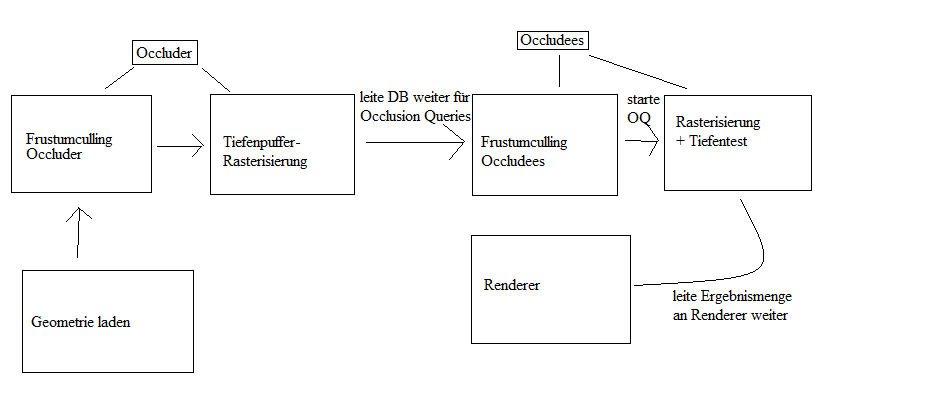
\includegraphics[width=\columnwidth]{images/SOCAblauf2.png}%
\caption{SOC-Ablauf: Nach Laden der Occludermenge wird im ersten Schritt durch Rasterisieren der Occluder der Tiefenpuffer generiert. Im zweiten Schritt werden die Occlusion Queries gestartet, die durch Rasterisierung und Tiefentests bestimmen, welche Objekte der Occludee-Menge sichtbar sind und welche nicht. Die Ergebnismenge wird an den Renderer weitergeleitet.}%
\label{fig:socablauf}%
\end{figure}


\subsection{Frustumculling}
Frustumculling l"asst nur Objekte passieren, die sich im Sichtbereich der Kamera befinden und kann somit je nach Kameraposition einen gro{\ss}en Teil der Objekte aus der Menge der zu rendernden Objekte herausnehmen. Daf"ur wird die AABB des Objekts gegen jede der sechs Ebenen des Frustums getestet, ob sich die AABB \textit{vollst"andig} au{\ss}erhalb einer dieser Ebenen befindet. Ist das der Fall, kann das Objekt als nicht sichtbar markiert werden und wird im weiteren Verlauf nicht weiter betrachtet. Dieser Zwischenschritt ist zwar optional, ist aber den Rechenaufwand wert, denn er bringt eine enorme Leistungssteigerung von teilweise "uber 100\%.\\
\textbf{(Optional! Vielleicht an anderer Stelle?)} Anmerkung zum Frustumculling: W"ahrend die Performance des Frustum Cullings sehr konstant bleibt, sind bei anderen Occlusion Culling Algorithmen gr"o\ss{}ere Schwankungen erkennbar, da ein gro\ss{}er Occluder im Vordergrund potenziell alle Occludees hinter ihm "uberdecken kann und damit die Berechnung stark vereinfacht \cite{MSOC}.\\


\subsection{Tiefenpuffer Rasterisierung}
Alle Occluder, die nach dem Frustumculling als sichtbar markiert sind, werden in diesem Schritt verwendet, um einen Tiefenpuffer zu generieren. Dazu werden alle sichtbaren Objekte als eine Occludermenge \glqq gerendert\grqq{} (es wird lediglich ein Tiefenpuffer erzeugt ohne die Objekte tats"achlich zu zeichnen). Das Rendering rasterisiert die Occluder, das hei{\ss}t, die Occluder werden auf den Bildschirm (screen space) transformiert und erzeugt anschlie{\ss}end den Tiefenpuffer, indem an den Stellen auf dem Bildschirm, an denen sich das Objekt befindet, die Tiefenwerte des Objekts gespeichert werden, siehe Abb.\ \ref{fig:db}.
\begin{figure}%
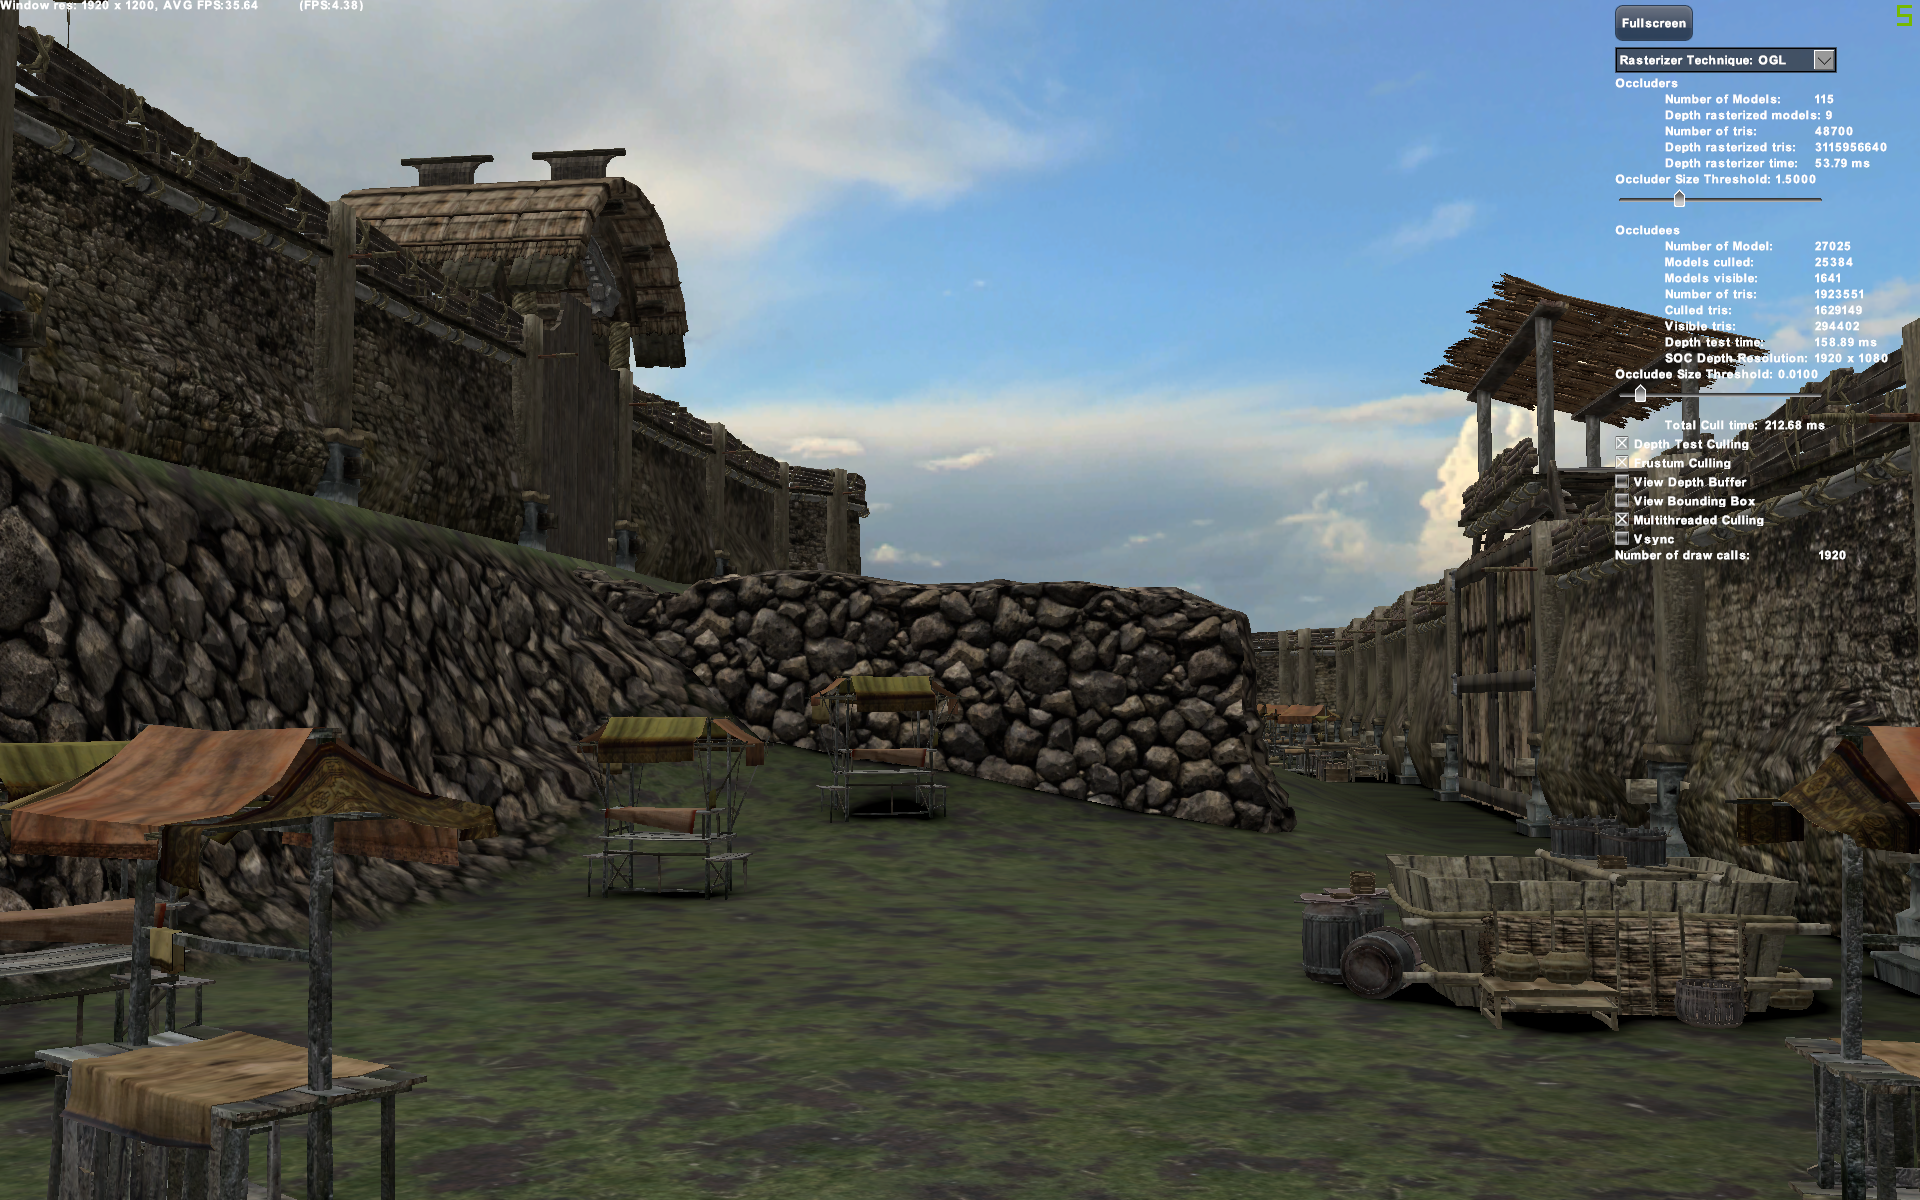
\includegraphics[width=0.5\columnwidth]{images/Base1.png}%
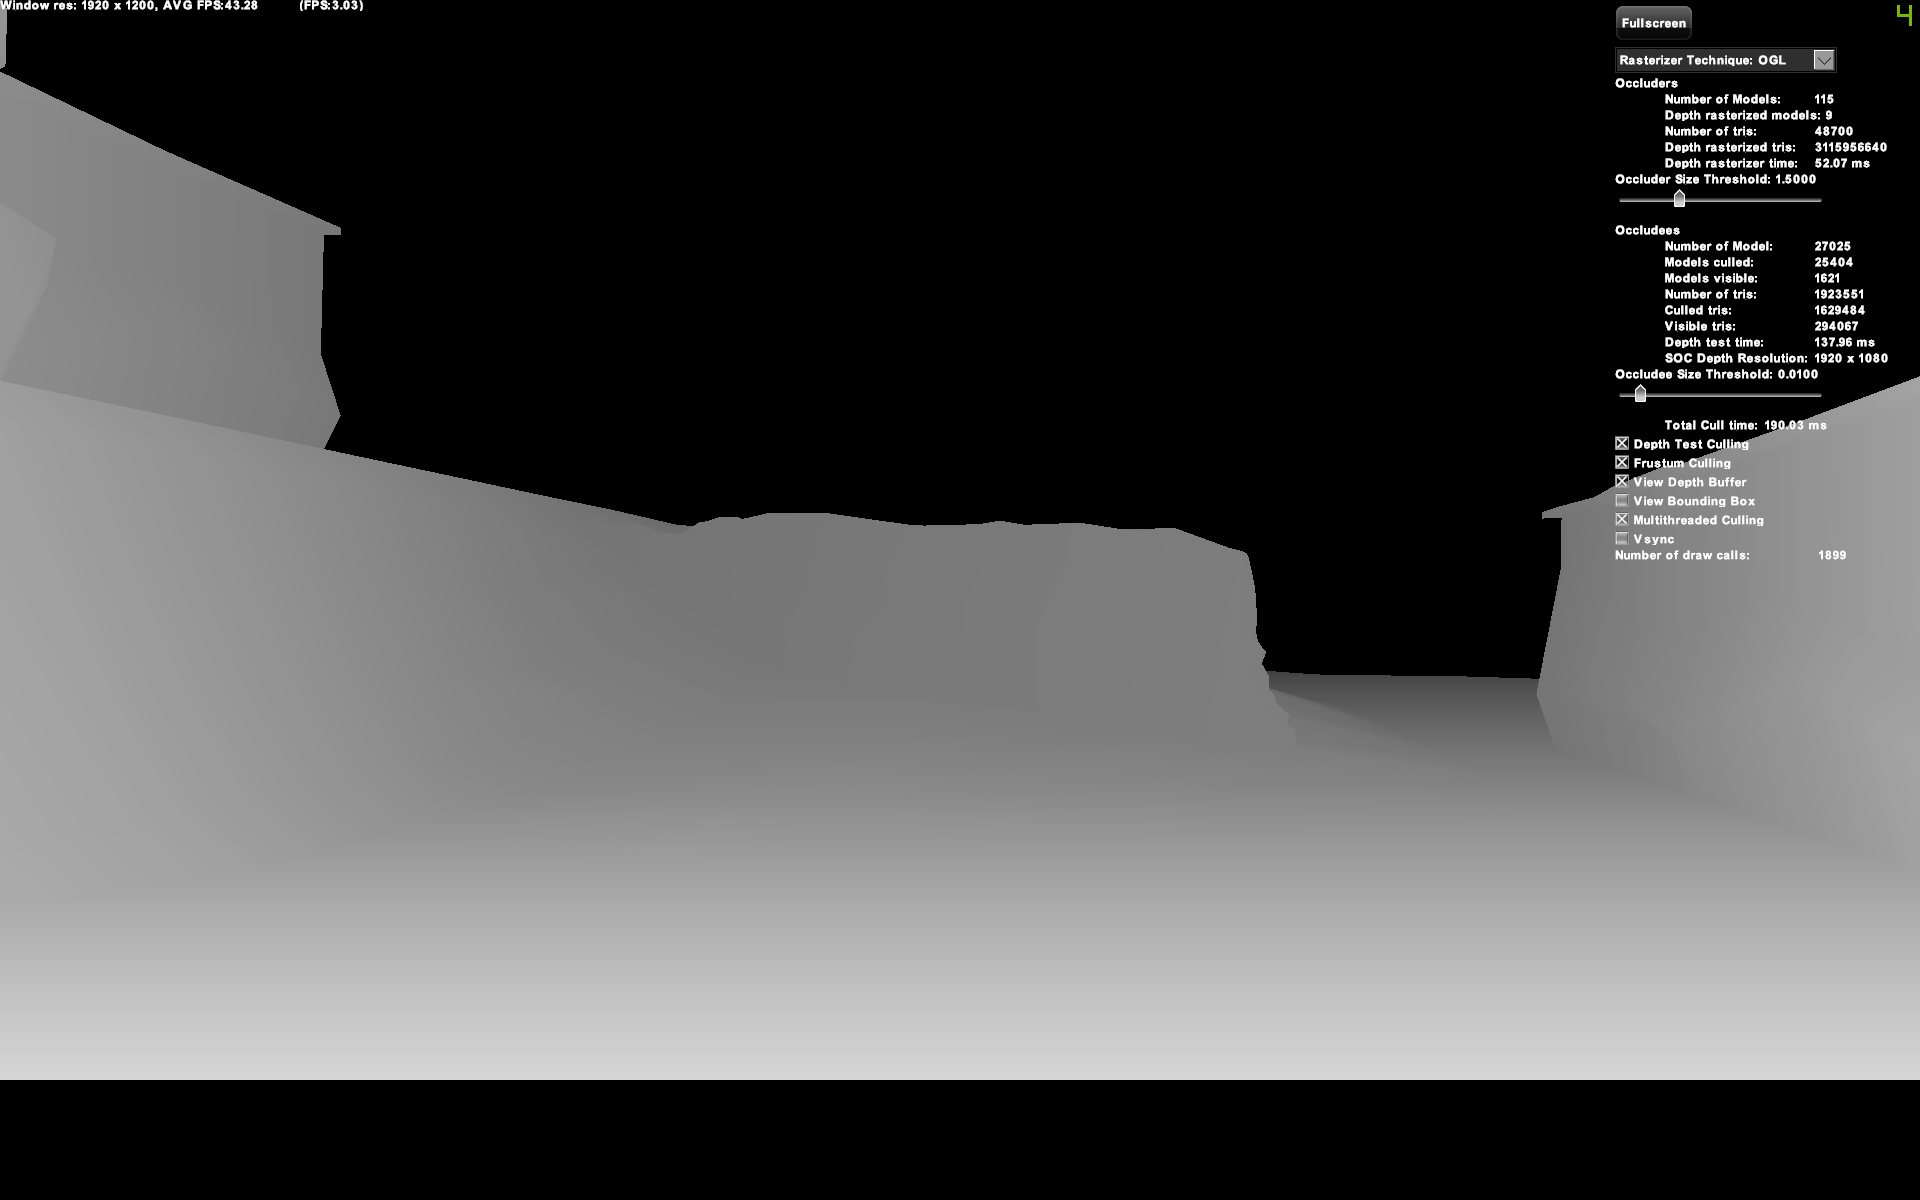
\includegraphics[width=0.5\columnwidth]{images/Base1DB.png}%
\caption{Links: Testbild der Szene. Rechts: Der dazugeh"orige Tiefenpuffer, der in jedem Frame einmal berechnet wird und sp"ater f"ur die Tiefentests der Occlusion Queries verwendet wird.}%
\label{fig:db}%
\end{figure}


\subsection{Occlusion Queries}
An dieser Stelle sei erw"ahnt, dass die gesamte Occludeemenge zu Beginn des Programms einmal hochgeladen wurde (wohin?) und im Programm selber nur via Indexlisten zugegriffen wird, so dass zus"atzliche Ladezeiten vermieden werden. Die Realisierung der Occlusion Queries gestaltet sich durch die von der OpenGL API zur Verf"ugung gestellten \textit{glQuery} sehr unkompliziert. Zu Anfang werden f"ur alle Occludees, die innerhalb des Frustums sind, eine Occlusion Query gestartet. Die Occludees werden wie die Occluder rasterisiert, allerdings wird in diesem Schritt der Tiefenpuffer nicht "uberschrieben, sondern es wird ausschlie{\ss}lich getestet, ob der Tiefenwert des Occludees kleiner als der des Tiefenpuffers ist. Die Occlusion Query testet also, ob ein Teil des Occludees bei einem potenziellen Renderdurchlauf sichtbar w"are. In diesem Fall liefert die Occlusion Query \glqq true\grqq{} zur"uck, andernfalls \glqq false\grqq{}. Nachdem alle Occlusion Queries ihre Berechnungen beendet haben, werden zum Schluss alle Ergebnisse abgefragt und an das Framework f"ur den weiteren Renderingverlauf weitergeleitet.


%%%%%%%%%%%%%%%%%%%%%%
%%%%% ERGEBNISSE %%%%%
%%%%%%%%%%%%%%%%%%%%%%
\section{Ergebnisse}
Probleme mit Occlusion Queries (lange Wartezeit bei Ergebnis holen), meiste Zeit in OQ --> Performanceverlust

Die dokumentierten Ergebnisse wurden mit dem SOC-Framework von Intel berechnet und verwenden die dortige Testszene einer Burg beziehungsweise eines Markplatzes, siehe Abb.\ \ref{fig:teaser}. Die Burg umfasst 115 Occluder mit 48700 Dreiecken und 27025  Occludees mit $\approx$ 1923000 Dreiecken. Sofern nicht anders angeben, wurden s"amtliche Ergebnisse mit einer Kamerafahrt, wie sie in Abb.\ \ref{fig:fahrt} angedeutet ist, "uber 100 Frames erstellt.
\begin{figure}%
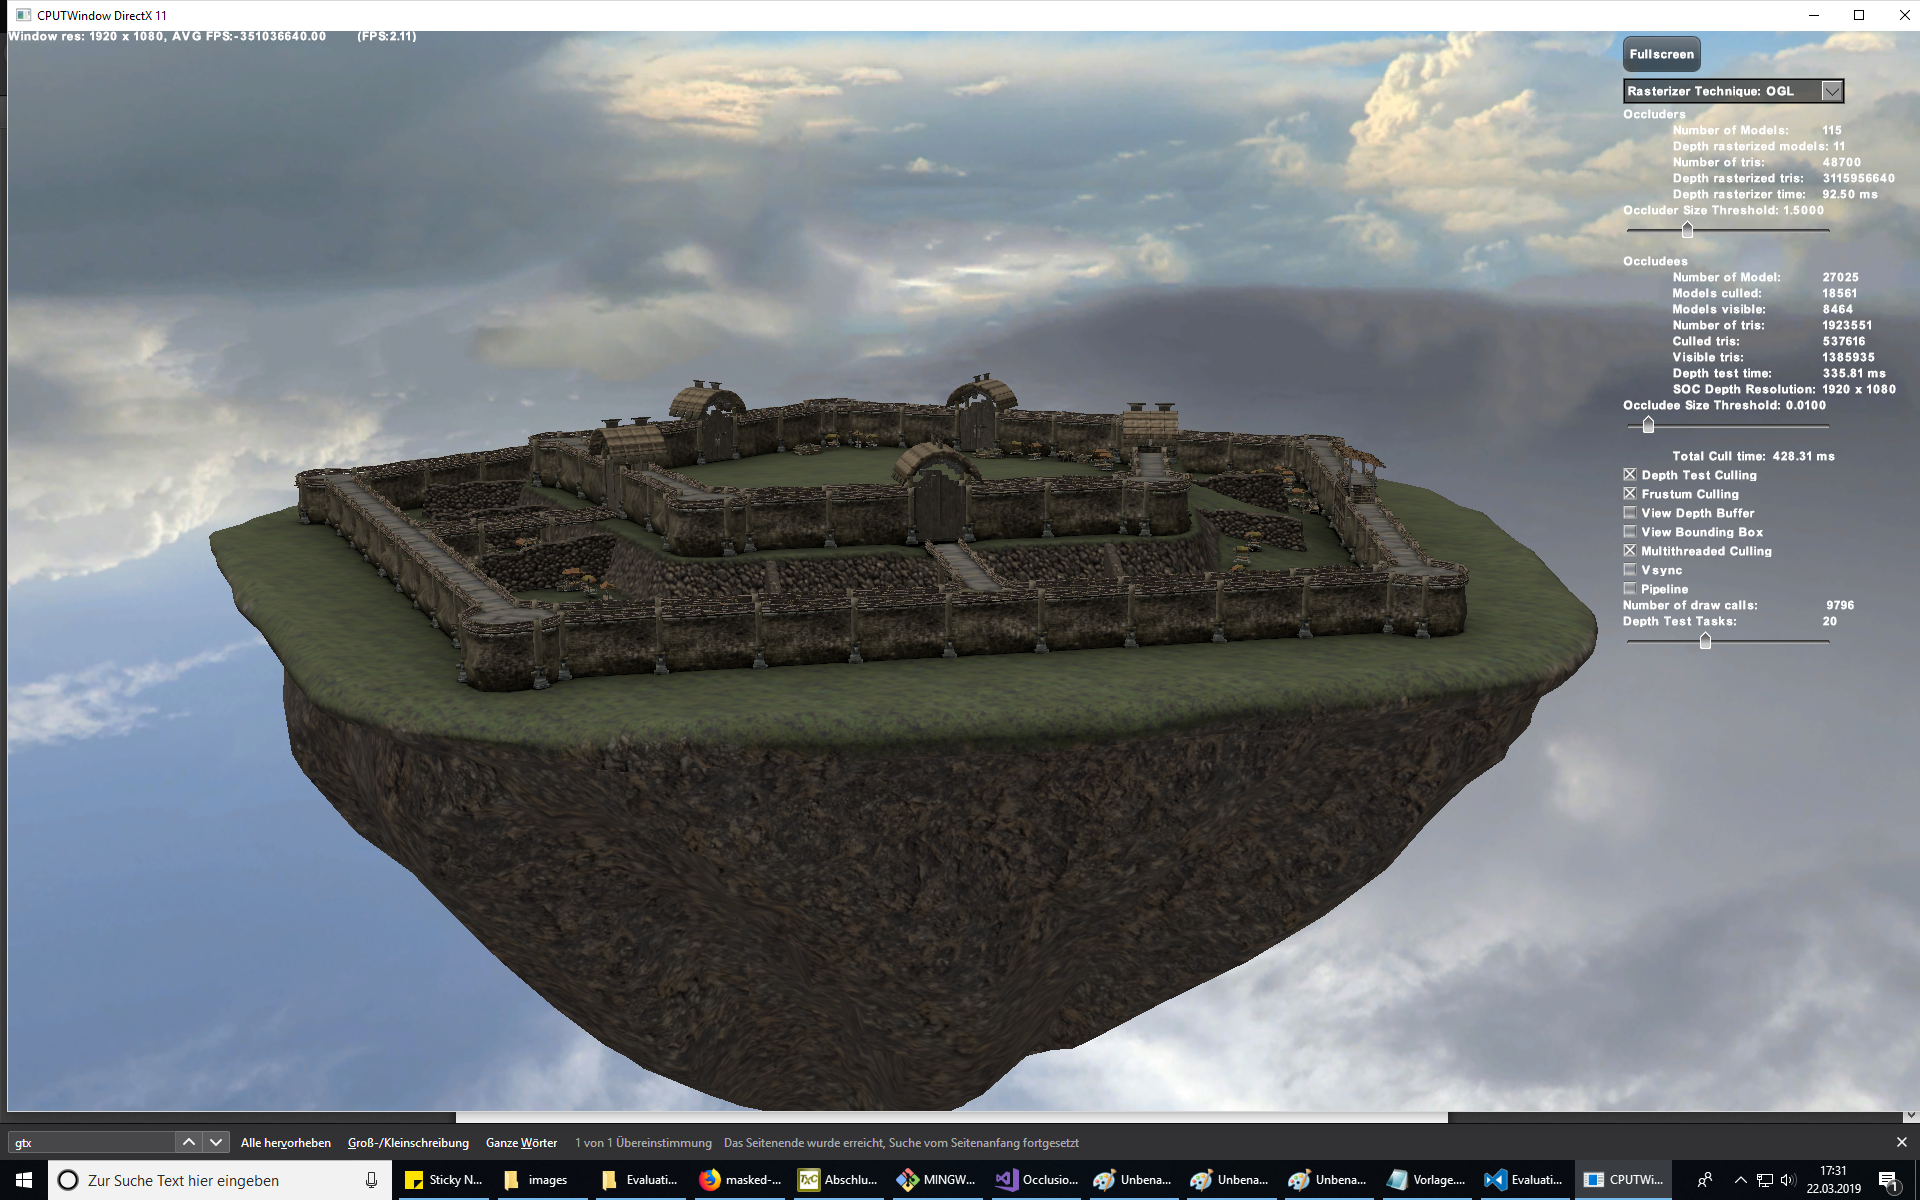
\includegraphics[width=0.33\columnwidth]{images/Tour1.png}%
\includegraphics[width=0.33\columnwidth]{images/Tour2.png}%
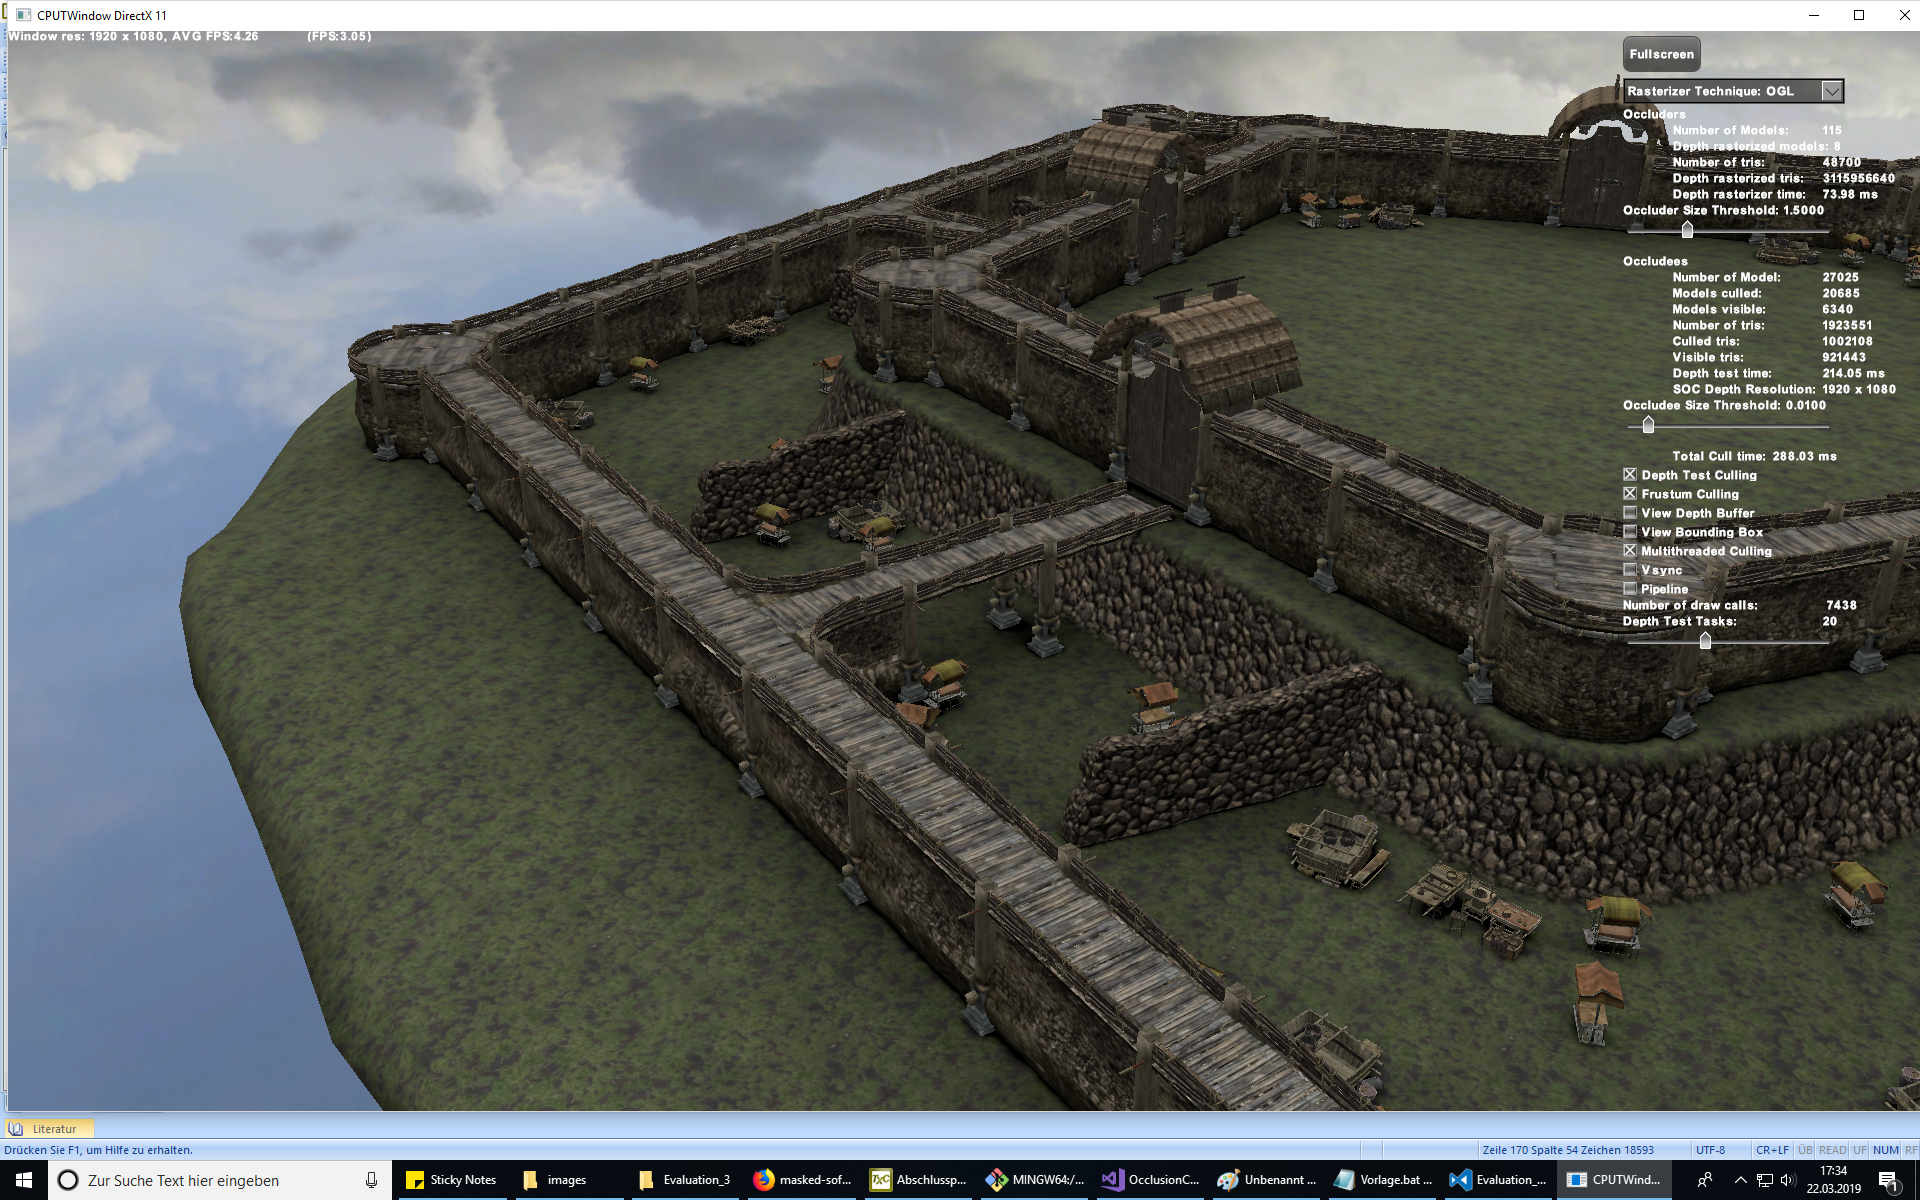
\includegraphics[width=0.33\columnwidth]{images/Tour3.png}%
\caption{Links: Startposition der Kamerafahrt. Mitte: n"ahert sich in einem Kreisbogen der Br"ucke an. Rechts: Die Kamera verl"asst die Szene in gleichem Bogen, wie sie sich angen"ahert hat.}%
\label{fig:fahrt}%
\end{figure}
Der Tiefenpuffer ist standardm"a"sig auf eine Aufl"osung von 1920x1080 Pixel gesetzt. Die Kamera startet mit Blick auf die Burg aus einiger Entfernung und fliegt auf die Burg zu. An der Burg angekommen dreht sich die Kamera in Richtung Boden und entfernt sich anschlie"send wieder von der Burg. Die Anzahl der Objekte im Sichtfeld ist am Anfang sehr hoch, sinkt in der Mitte der Kamerafahrt ab und steigt am Ende wieder auf den Startwert. Als Hardware wurde ein Rechner mit einem Intel Core i9-7900X, einer NVIDIA Titan Xp und 64 GB RAM verwendet.

\begin{figure*}
	\begin{minipage}{\textwidth}
		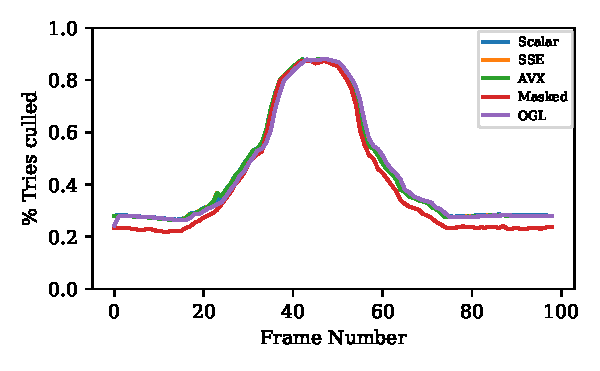
\includegraphics[width=0.5\textwidth]{images/Evaluation_1_Results_Percentage culled.pdf}
		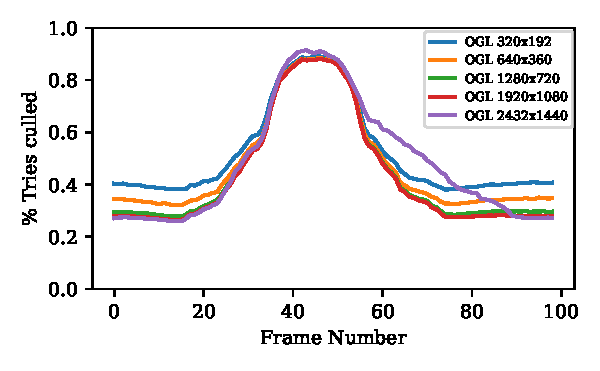
\includegraphics[width=0.5\textwidth]{images/Evaluation_4_Results_Percentage culled.pdf}
	\end{minipage}
	\begin{minipage}{\textwidth}
		\centering
		\scalebox{1.2}{
			\begin{tabular}{| l | r | r | r | r | r | r |}
				\hline
				& 320x192   & 640x360   & 1280x720  & 1920x1080 & 2432x1440 & 3840x2160 \\ \hline
				Tries culled (\%)    & 51.88     & 47.65     & 44.69     & 43.81     & 48.55     & 75.03     \\ \hline
				Draw Calls           & 3640      & 5759      & 7725      & 8515      & 7920      & 2602      \\ \hline
				Models Culled        & 23795.46  & 21996.8   & 20346.68  & 19683.44  & 20196.8   & 24718.0   \\ \hline
				Models Visible       & 3229.54   & 5028.2    & 6678.32   & 7341.56   & 6828.2    & 2307.0    \\
				\hline
		\end{tabular}}
	\end{minipage}
	\caption{Im linken Diagramm ist die Prozentangabe der gecullten Dreiecke mit den f"unf verschiedenen 	Methoden, bei einer Aufl"osung des Tiefenbuffers von 1920x1080, zu sehen.
		Im rechten Diagramm wird die Anzahl der gecullten Dreiecke bei unserer OGL Methode mit f"unf verschiedenen Aufl"osungen des Tiefenbuffers verglichen.}
	\label{fig:resolution_culled}
\end{figure*}

\begin{figure*}
	\begin{minipage}{0.4\textwidth}
		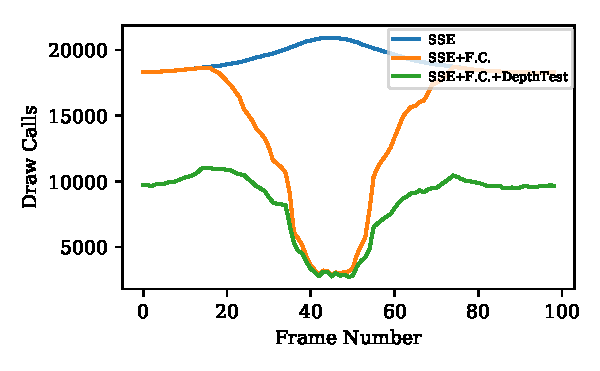
\includegraphics[width=\textwidth]{images/Evaluation_7_Results_SSE_Draw Calls.pdf}
	\end{minipage}
	\begin{minipage}{0.4\textwidth}
		\centering
		\scalebox{1.2}{
			\begin{tabular}{| l | r | r | r | r | r |}
				\hline
				& MT        & MT+Frustum& MT+Frustum\\
				&           &           & + Depth Test\\ \hline
				Tries culled (\%)    & 11.13     & 11.13     & 43.88     \\ \hline
				Draw Calls           & 19219     & 14318     & 8442      \\ \hline
				Models Culled        & 10180.34  & 14532.39  & 19728.07  \\ \hline
				Models Visible       & 16844.66  & 12492.61  & 7296.93   \\
				\hline
		\end{tabular}}
	\end{minipage}
	
	\begin{minipage}{0.4\textwidth}
		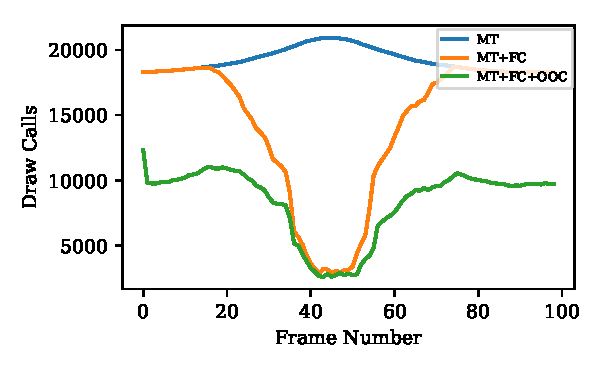
\includegraphics[width=1\textwidth]{images/Evaluation_7_Results_OGL_Draw Calls.pdf}
	\end{minipage}
	\begin{minipage}{0.4\textwidth}
		\centering
		\scalebox{1.2}{
			\begin{tabular}{| l | r | r | r | r | r |}
				\hline
				& MT        & MT+Frustum& MT+Frustum\\
				&           &           & + Depth Test\\ \hline
				Tries culled (\%)    & 11.13     & 11.13     & 43.81     \\ \hline
				Draw Calls           & 19219     & 14318     & 8515      \\ \hline
				Models Culled        & 10180.34  & 14532.39  & 19683.44  \\ \hline
				Models Visible       & 16844.66  & 12492.61  & 7341.56   \\
				\hline
		\end{tabular}}
	\end{minipage}
	\caption{Vergleich von Multi-Threading (MT), MT + Frustum Culling und MT + Frustum Culling + Depth Test Culling. Oben sie die Ergebnisse des MOC zu sehen, unten die unserer OGL Methode. !!! Im Moment noch SSe statt MOC !!!}
	\label{fig:OGL_MOC_frustum_culling}
\end{figure*}

\begin{figure*}
	\begin{minipage}{\textwidth}
		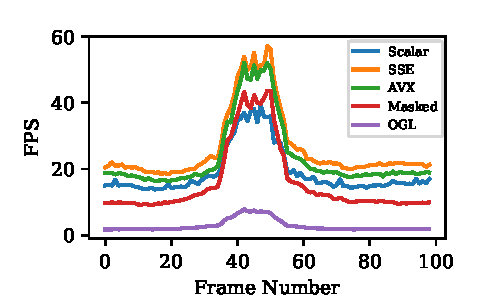
\includegraphics[width=0.5\textwidth]{images/Evaluation_1_Results_FPS.pdf}
		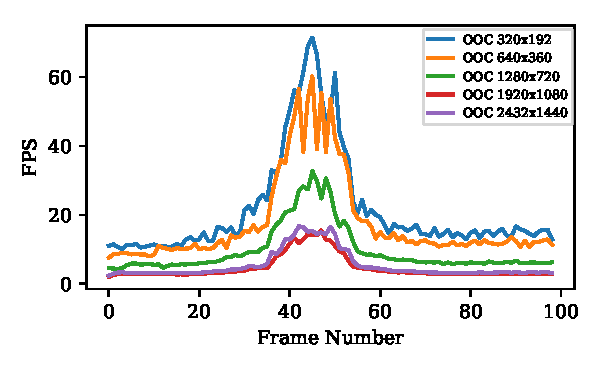
\includegraphics[width=0.5\textwidth]{images/Evaluation_4_Results_FPS.pdf}
	\end{minipage}
	\begin{minipage}{\textwidth}
		\centering
		\scalebox{1.2}{
			\begin{tabular}{| l | r | r | r | r | r | r |}
				\hline
				& 320x192   & 640x360   & 1280x720  & 1920x1080 & 2432x1440 & 3840x2160 \\ \hline
				FPS                  & 5.87      & 5.33      & 4.6       & 3.55      & 3.46      & 3.81      \\ \hline
				DepthTest time (ms)  & 112.33    & 124.68    & 157.83    & 235.25    & 245.85    & 236.42    \\ \hline
				Rasterize time (ms)  & 63.3      & 63.97     & 62.43     & 63.46     & 66.34     & 63.93     \\
				\hline
		\end{tabular}}
	\end{minipage}
	\caption{Im linken Diagramm die FPS der f"unf verschiedenen Methoden, bei einer Aufl"osung des Tiefenbuffers von 1920x1080, zu sehen.
		Im rechten Diagramm wird die Anzahl der FPS bei unserer OGL Methode mit f"unf verschiedenen Aufl"osungen des Tiefenbuffers verglichen.}
	\label{fig:resolution_fps}
\end{figure*}

%Notizen zu den Ergebnissen:
%%%%%%%%%%%%%%%%%%%%%%%%%%%%%%%%%%%%%%%%%%%%%%
%Evaluation 1: alle 5, Kamerafahrt 1\\
%Evaluation 2: alle 5, Kamerafahrt 2\\
%Evaluation 3: alle 5, DB\_Very\_Large vs DB\_Small\\
%Evaluation 4: OGL, alle 5 Aufl"osungen\\
%Evaluation 5: OGL, mit und ohne Frustum culling\\
%Evaluation 6: alle 5 + OGL ohne Mesa\\
%Evaluation 7: OGL + SSE, MT / MT + Frustum Culling / MT + Frustum Culling + Depth Test Culling\\
%Evaluation 8: OGL + SSE, Depth Test Tasks 5 / 20 / 100
%
%1)
%- Auflösungen DB
%- Diagramm: Percentage culled Evaluation 1 + 4 nebeneinander
%- Tabelle: \% Culled, Drawcalls, Models Culled, Models Visible
%
%2)
%- MT/MT+Frustum/MT+Frustum/DP
%- Diagramm: Drawcalls OGL + MOC
%- Tabelle: Models Visible, Models Culled, Drawcalls, \% Culled tries
%
%3)
%- Auflösungen DB
%- Diagramm: Frames alle
%- Diagramm: Frames OGL Auflösungen
%- Tabelle:  Frames, DT time, Rasterizer time
%
%Optional:
%5)
%- Future Work
%- Mehrere Occluder gleichzeitig rendern 
%6) OGL vs ohne Mesa
%7) Depth Test Task 1-100
%8) Occluder Threshold
%9) Occludee Threshold
%%%%%%%%%%%%%%%%%%%%%%%%%%%%%%%%%%%%%%%%%%

\section{Fazit}
Das ist ein Testsatz f"ur das Fazit.

\section{Future Work}
Occludee zu Paketen schn"uren und als Paket hochladen. Ziel ist es, weniger Occlusion Queries bei gleichem Ergebnis zu generieren und dadurch an Performance zu gewinnen.
Auswahl der Occludee, die zu einem Paket zusammengeschn"urt werden ist dabei von gro"ser Wichtigkeit und entscheidend f"r das Ergebnis, sowohl im Hinblick auf die Performance, als auch auf die Korrektheit des Ergebnisses (werden alle Occludee angezeigt, die sichtbar sind oder fehlen offensichtliche Objekte in der Szene).

\bibliographystyle{abbrv} 
%% use following if all content of bibtex file should be shown
% \nocite{*}
\bibliography{literatur}
\end{document}
